\usepackage[14pt]{extsizes}
\documentclass[a4paper,14pt]{article}
\usepackage{maicoursework}
\usepackage{float}
\makeglossaries

\newacronym{api}{API}{Applicatoin Programming Interface}
\newacronym{rest}{REST}{Representational State Transfer}
\newacronym{spa}{SPA}{Single Page Application}
\newacronym{mvc}{MVC}{Model View Controller}
\newacronym{orm}{ORM}{Object-Relational Mapping}
%%% Преамбула
\author{Солдатов Вячеслав Алексеевич}
\title{Паттерны проектирования}
\date{}
\MAIProfessorName{Романенков Александр Михайлович}
\MAIWorkType{Курсовая работа}
\MAISubject{Фундаментальные алгоритмы}
\MAIGroup{М80-211Б-19}
\begin{document}

\maketitle
\setcounter{page}{2}
\tableofcontents
\clearpage
\clearpage


\section{Описание задания}
\subsection{Вариант №32}
Разработайте приложение для проведения лотереи (например, аналога
Русского лото). Ваше приложение должно обеспечивать генерацию билетов для
очередного тиража лотереи (генератор должен быть реализован посредством
паттерна “фабричный метод”). Количество генерируемых билетов произвольно и
может быть велико (> 20’000’000 шт.). Учтите ситуацию, что не все
сгенерированные билеты могут участвовать в тираже (это типичная ситуация,
которая возникает при неполной реализации билетов к тиражу). Смоделируйте
проведение розыгрыша: на каждом ходе проверяйте, появился ли победитель;
предусмотрите систему выигрышей; предоставьте возможность поиска билетов
по заданным критериям: номеру билета, величине выигрыша, и т. д.. Сохраняйте
информацию о проведенных тиражах для обеспечения поиска данных в
будущем. Реализуйте функционал обработки данных таким образом, чтобы тип
коллекции, в которой будут храниться ваши данные, являлся параметром.
Продемонстрируйте обработку данных с использованием std::forward\_list и
собственной реализации односвязного списка.
\clearpage

\section{Описание решения}

\subsection{Описание алгоритма}
Для решения поставленной задачи программа выполняет следующие действия\newline
\begin{enumerate} 
  \item Открытие файла на запись с проверкой. Если проверка не пройдена, программа завершает свою работу с кодом ошибки, переданным в функцию errCheck\_Main(), которая также выводит информацию для пользователя в соответствии с кодом ошибки.
  \item Передача управления функции clientCode()
  \item Создание генераторов для генерации обьектов типа: БИЛЕТ, ТИРАЖ, ИГРА.
  \item Создание объекта класса ИГРА, ввод пользователем следующих параметров: id игры, количество тиражей, количество билетов в каждом тираже, шанс продажи билета.
  \item Создание объектов класса ТИРАЖ внутри конструктора класса ИГРА с помощью генератора, помещение объектов класса ТИРАЖ в односвязный список указателей типа ТИРАЖ - приватное поле класса ИГРА. 
  \item Создание объектов класса БИЛЕТ, внутри конструктора класса ТИРАЖ с помощью генератора, помещение объектов класса БИЛЕТ в односвязный список указателей типа БИЛЕТ - приватное поле класса ТИРАЖ. 
  \item Возвращение управления функции clientCode(), начало взаимодействия с пользователем в формате "ввод операции - вывод данных или особого ответа."
  \item При вводе пользователем операции обработки игры происходит обработка тиража, номер которого указал пользователь, или всех тиражей с помощью функции processGame().
  \item Передача управления функции processLot().
  \item В функции processLot() происходит "пошаговая" обработка билетов по принципу: вынимается бочонок с числом - обрабатывается весь список билетов. Если число на боченке совпадает с числом в одном или нескольких из полей билета, число в билете "зачеркивается".
  \item Выбор победителей посредством проведения 3-х туров. Билет выйгравший в определенном туре помечается особым образом и попадает в список указателей <имя тура>\_tour\_winner\_tickets типа БИЛЕТ - приватное поле класса ИГРА.
  \item Возвращение управления функции processGame(), внутри которой сначала происходит обработка ошибок с помощью функций заголовочного файла error\_check.h, которые могли возникнуть при обработке тиражей в функции processLot.
  \item В функции processGame() происходит вывод всех списков с названиями  <имя тура>\_tour\_winner\_tickets в стандартный поток вывода, таким образом показывая пользователю победившие билеты.
  \item Возвращение управления функции clientCode() вместе с кодом ошибки, обработка ошибок с помощью функций заголовочного файла error\_check.h, блокирование доступа к определенным операциям в завсисмости от кода ошибки.
  \item Следующая итерация взаимодействия с пользователем, в зависимости от введенной пользователем операции производится вывод данных об прошедшей игре в файл, поиск билета по файлу.
  \item Завершение работы с пользователем, очистка памяти.
  \item Возвращение управления функции main() вместе с кодом ошибки, обработка ошибок с помощью функций заголовочного файла error\_check.h, завершение работы программы с помощью функции errCheck\_Main().
\end{enumerate}
\subsection{Описание реализованных сущностей}
Для решения поставленной задачи были реализованы следующие сущности:
\subsubsection{main.cpp}
\begin{center}
   Функция main()
\end{center}
Открывает файл output\_file.txt на запись 
\item Задает seed для случайно генерации чисел в объектах класса ПОЛЕ - приватных объектах класса БИЛЕТ
\item Передает управление функции clientCode()
\item Обрабатывает код ошибки, полученный в качестве возвращаемого значения от функции clientCode(), передавая управление функции  errCheck\_Main().
\subsubsection{client\_code.h}
\begin{center}
   Функция clientCode()
\end{center}
Создает указатели на объекты классов SuperGenerator и Game
\item Осуществляет взаимодействие с пользователем с помощью классической контрукции while(true) и switch(operation). Доступные для пользователя операции: p - основная операция, выявление победителей среди купивших билет, обработка тиражей; о - вывод данных всех по проведенной игре в файл output\_file.txt; s - поиск определенного билета в файле output\_file.txt; с - выход из цикла, завершение взаимодействия с пользователем.
\item Очистка памяти.
\subsubsection{functions.h}
\begin{center}
   Функция floatChanceToInt(float)
\end{center}

Приведение пользовательского значения типа float к значению типа int. Используется для получения шанса продажи билетов для тиража.
\newpage
\begin{center}
   Функция foundDuplicate(int8\_t*, int, int)
\end{center}

Поиск дубликатов в массиве, замена дубликата другим значением
\begin{center}
   Функция getValues(int8\_t*)
\end{center}

Заполнение массива размером 2х5 случайными значениями, используется функция foundDuplicate().
\subsubsection{components.h}
Все классы, кроме класса KegBag, описанные в этом заголовочном файле, имеют вроизводные классы с приставкой RusLot в названии.
\begin{center}
   Класс KegBag
\end{center}

Задача этого класса - симуляция мешка с бочонками. Количество бочонков задается макросом NUMBER\_OF\_KEGS и специально сделано неизменяемым с пользовательской стороны. Класс имеет метод для вытаскивания одного бочонка или нескольких бочонков getKegs(vector<unsigned int>&, unsigned int), а также оператор вывода в поток.
\begin{center}
   Абстрактный класс Field
\end{center}

Этот класс содержит указатель на указатель типа unsigned int8\_t, количество строк и столбцов поля билета, имеет перегруженный деструктор для очистки памяти, операторы выгрузки и вставки в поток. Класс Ticket является дружественным к этому классу.
\begin{center}
   Шаблонный абстрактный класс Ticket
\end{center}

Этот класс содержит шаблонный вектор полей производного класса от класса Ticket, а также поля атомарных типов для вывода информации о билете. Имеет метод getStatus() нужный для получения информации о статусе билета (продан, куплен, победил в n-ом туре и т.д.), processTicket(), который "зачеркивает" совпавшие числа в полях билета, имеет операторы вставки и выгрузки из потока. Абстрактный класс Lot и шаблонная функция Ticket<> *searchTickets(Game<, >&, Ticket<>*, int) являются дружественными к этому классу.
\begin{center}
   Шаблонный абстрактный класс Lot
\end{center}

Этот класс хранит список указателей на объекты класса Ticket, объект класса KegBag, оператор выгрузки из потока. Абстрактный шаблонный класс Game является дружественным к этому классу.
\begin{center}
   Шаблонный абстрактный класс Game
\end{center}

Этот класс хранит список указателей на объекты класса Lot, а также три списка указателей на объекты класса Ticket. Класс Game в самом верху иерархии лотереи, имея список класса Lot (тираж). Конструктор класса, используя методы класса, создает лотерию, иерархично создавая объекты классов типа Lot и Ticket. Game имеет методы вывода в стандартный поток списков билетов-победителей printWinners(ListBasicInterface< , Ticket<>*>&), задания пользователем параметров генерации тиражей и билетов generationMenu(), генерации тиражей generationProceed(float, GeneratorLot<T, L>&, GeneratorTicket<T>&), обработки тиража processLot(long int, auto lot) и всей игры processGame(int, unsigned int, int), проведения розыгрыша processTour(unsigned int, auto& lot, ListBasicInterface< , Ticket<>*>&, int, vector<unsigned int>&), вставки в поток.
\subsubsection{generators.h}
В этом файле хранятся абстрактные шаблонные и производные генераторы для всех классов, кроме Field и KegBag. При генерации билетов используется паттерн "Фабричный метод".Также здесь определен абстрактный класс SuperGenerator, хранящий указатели на абстрактные шаблонные генераторы.
\subsubsection{err\_check.h}
В этом файле хранятся хранятся функции int errCheck\_Components(int, unsigned int), int errCheck\_ClientCode(int, long int), int errCheck\_Main(int, long int) для обработки ошибок на разных уровнях выполнения программы.
Реализация одной из функций:
\begin{minted}{C++}
int errCheck_Components(unsigned int additional_information)
{
    switch(err_code)
    {
        case 1:
            cerr << NON_CRITICAL"Unable to find Lot with id " << additional_information << " in Game!\nProcessing of this lot will not begin.\n\n";
            break;
        case 2:
            cerr << NON_CRITICAL"Lot with id " << additional_information << " has been already processed.\nReprocessing is prohibited\n\n";
            break;
    }
}
\end{minted}
\subsubsection{list\_decorator.h}
В этом файле хранится реализация собственного односвязного списка в виде класса List со стандартными для односвязного списка методами и общий для List и forward\_list шаблонный интерфейс в виде класса ListBasicInterface, хранящий контейнер односвязного списка.

\begin{center}
    \subsubsection{Структура билета}
\end{center}
Билет содержит поля:
\begin{enumerate} 
  \item Номер тиража
  \item Номер билета
  \item Статус билета
  \item Вектор, содержащий игровые поля.
\end{enumerate}

\clearpage
\begin{center}
    \subsubsection{Демонстрация работы, входные и выходные данные}
\end{center}

\begin{figure}[H]
  \centering
  \captionsetup{justification=centering,margin=1cm}
  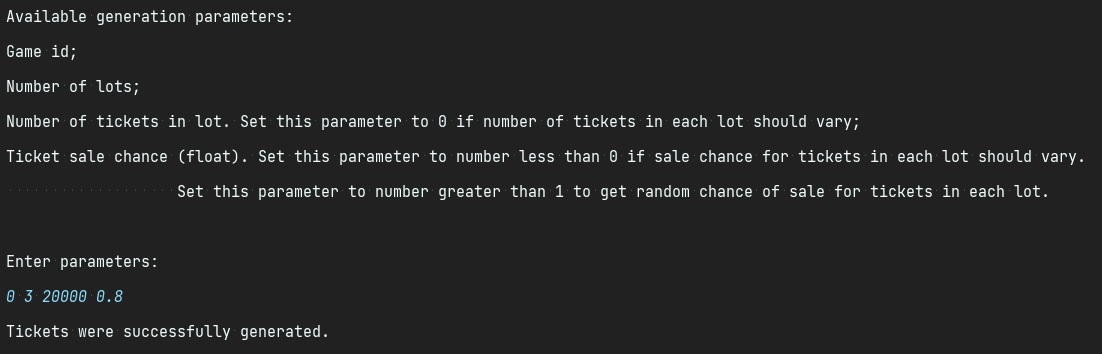
\includegraphics[width=\linewidth]{pictures/9}
  \caption{Пользователь вводит собственные параметры для генерации тиражей.}
\end{figure}
\begin{figure}[H]
  \centering
  \captionsetup{justification=centering,margin=1cm}
  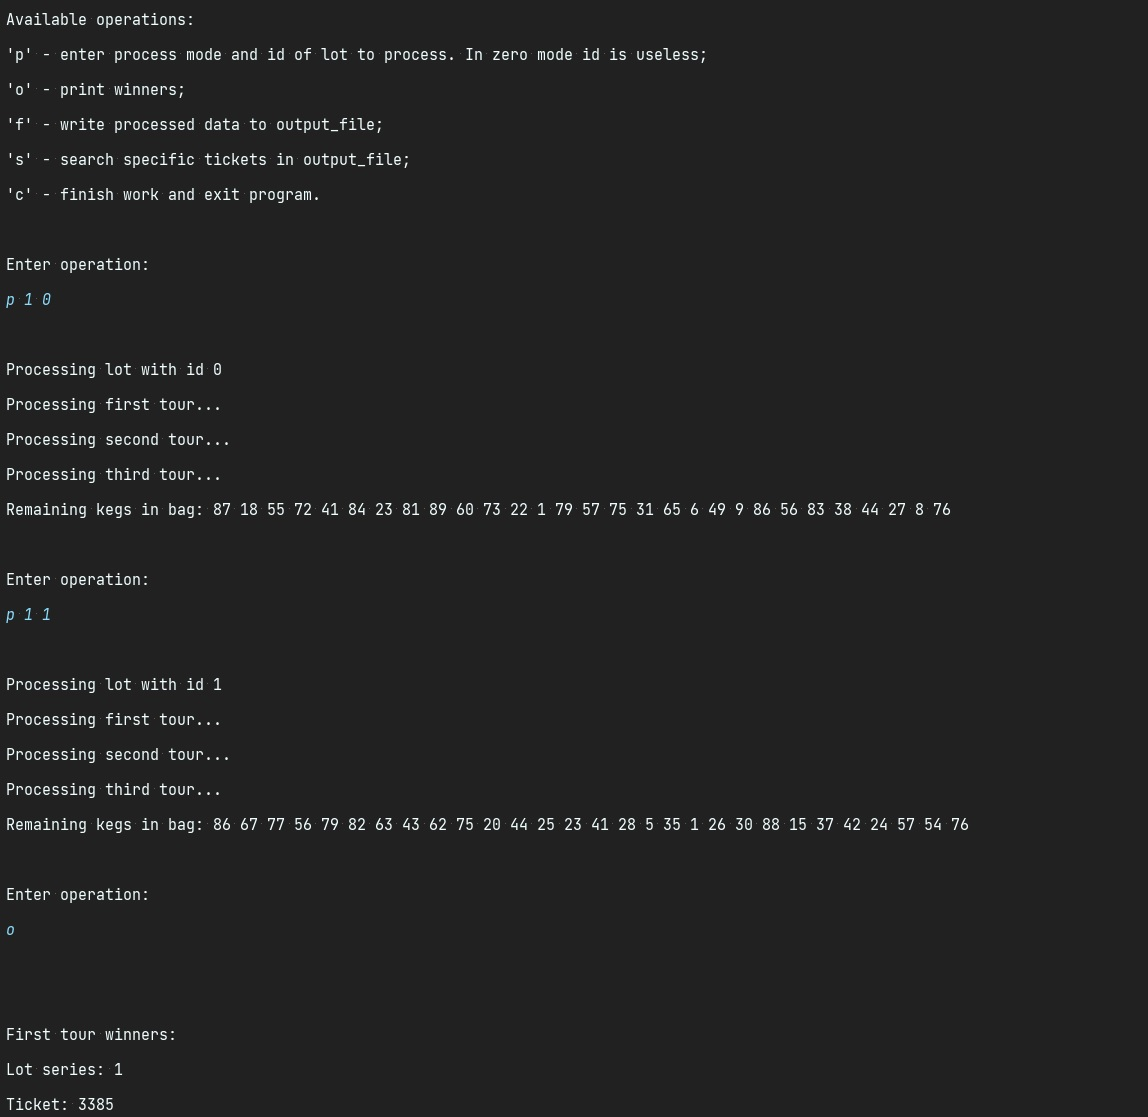
\includegraphics[width=\linewidth]{pictures/1}
  \caption{Пользователь вводит операцию обработки первого и второго тиража билетов, и операцию вывода победитлей в стандартный поток. Программа обрабатывает тиражи без ошибок.}
\end{figure}
\begin{figure}
  \centering
  \captionsetup{justification=centering,margin=1cm}
  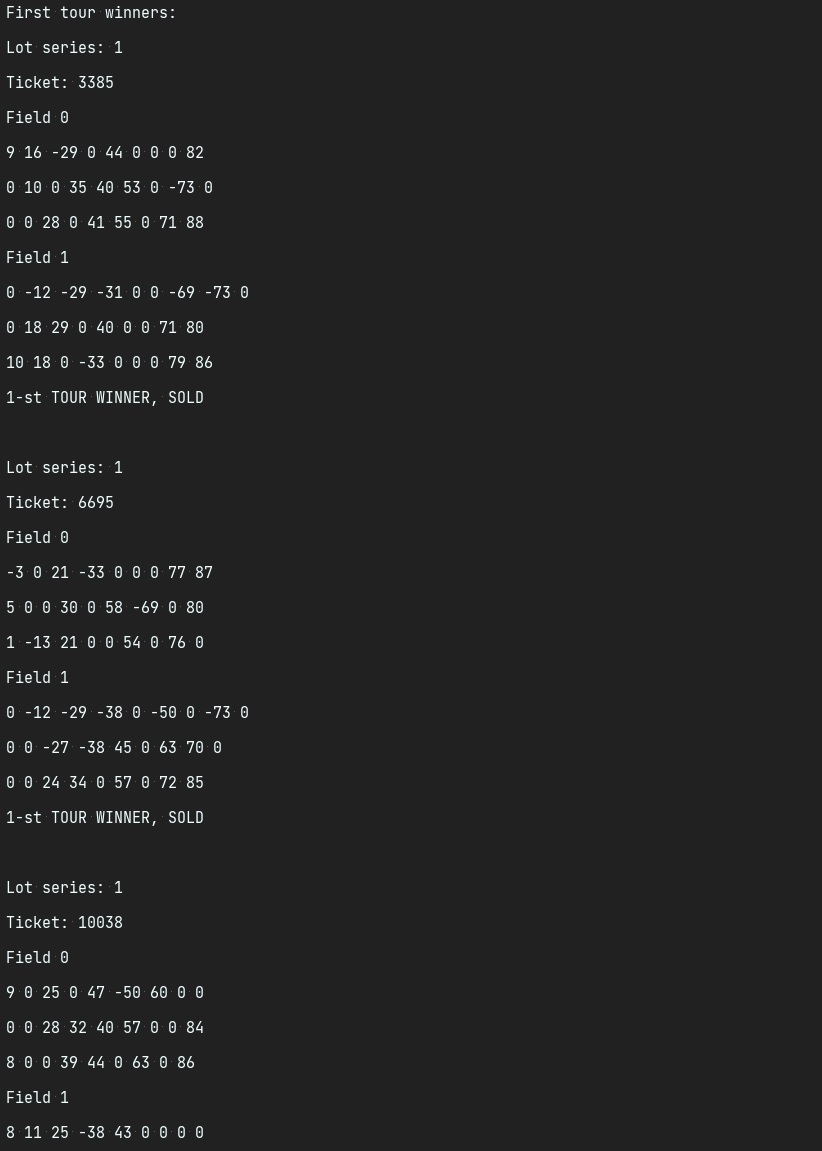
\includegraphics[width=\linewidth]{pictures/2}
  \caption{Программа выводит в стандартный поток вывода билеты, победившие в первом туре.}
\end{figure}
\begin{figure}
  \centering
  \captionsetup{justification=centering,margin=1cm}
  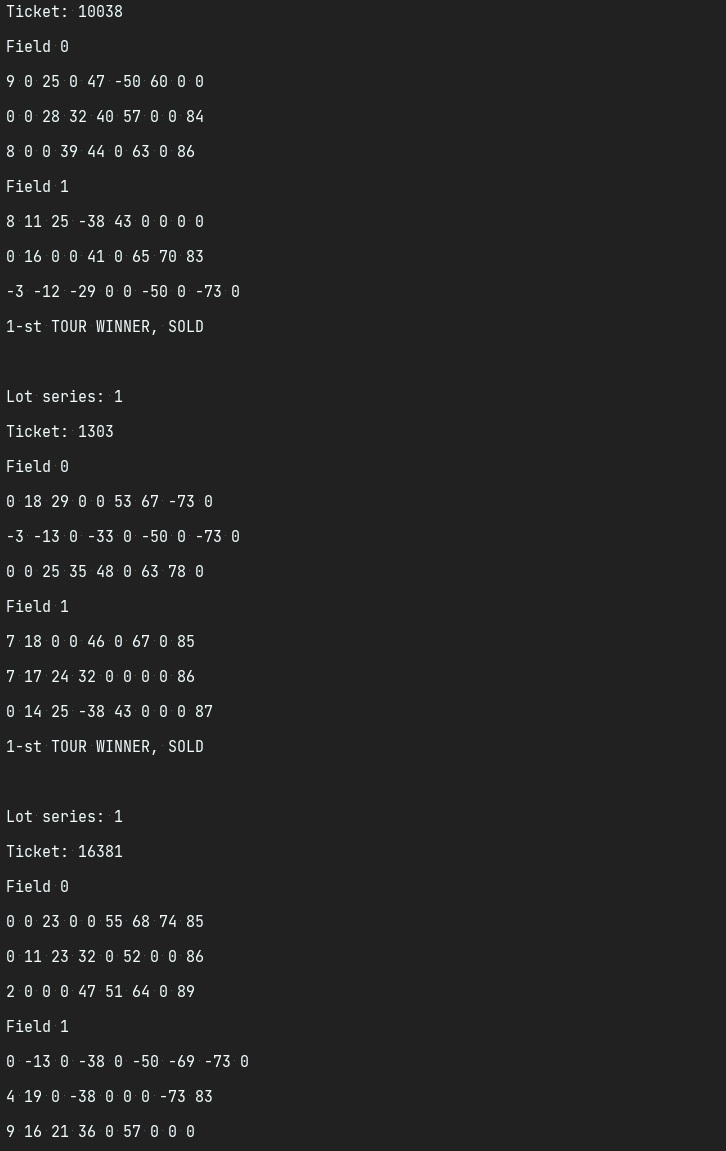
\includegraphics[scale=.95]{pictures/3}
  \caption{Программа выводит в стандартный поток вывода билеты, победившие в первом туре.}
\end{figure}
\begin{figure}[H]
  \centering
  \captionsetup{justification=centering,margin=1cm}
  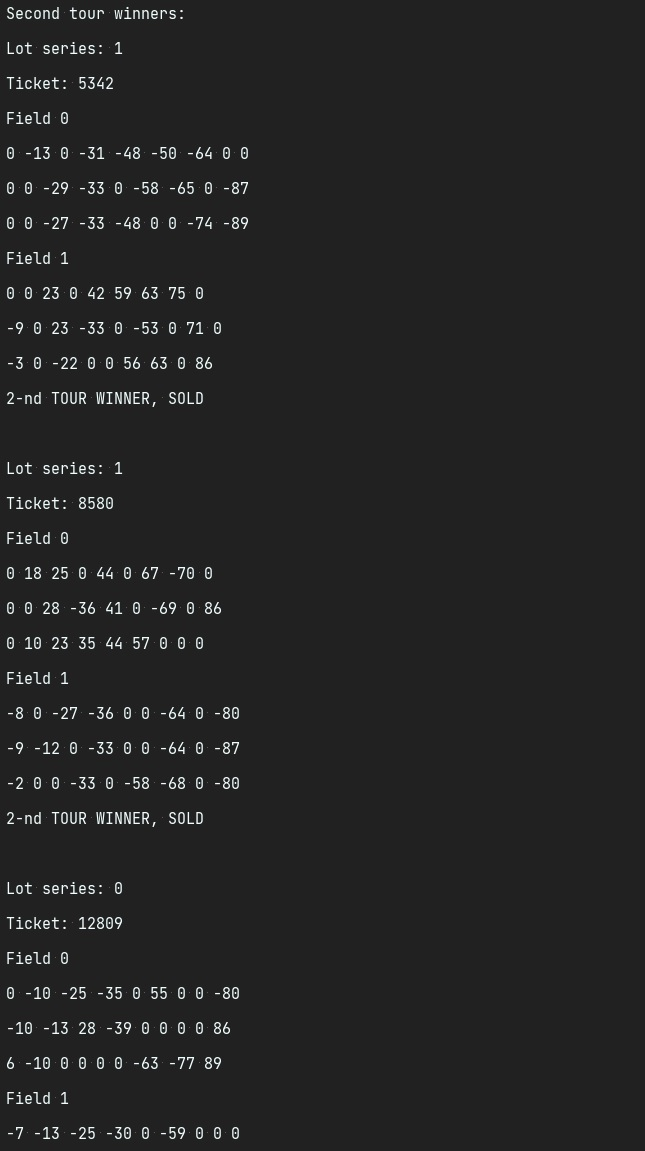
\includegraphics[scale=.95]{pictures/4}
  \caption{Программа выводит в стандартный поток вывода билеты, победившие во втором туре.}
\end{figure}
\begin{figure}
  \centering
  \captionsetup{justification=centering,margin=1cm}
  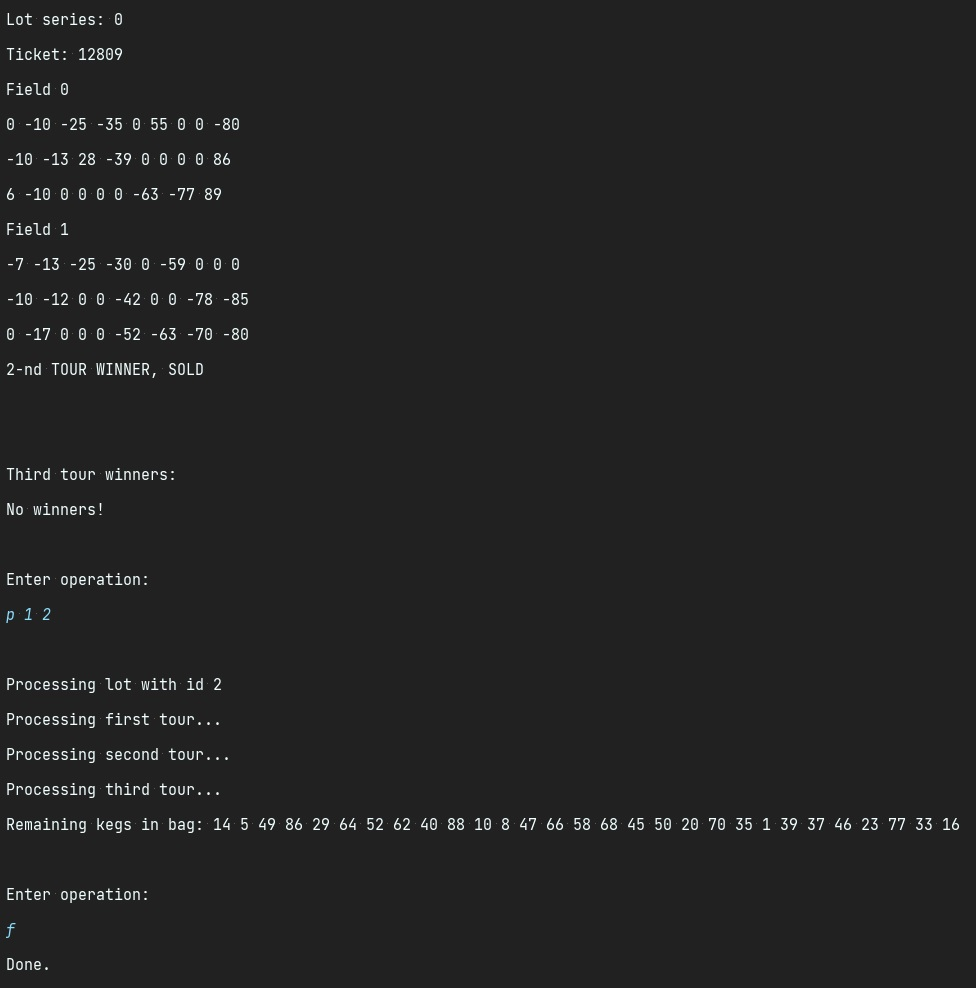
\includegraphics[width=\linewidth]{pictures/5}
  \caption{Программа закончила вывод победивших во втором туре билетов и сообщила, что победителей в третьем туре нет. Пользователь вводит операцию обработки третьего, последнего тиража и операцию вывода данных в файл.}
\end{figure}
\begin{figure}[H]
  \centering
  \captionsetup{justification=centering,margin=1cm}
  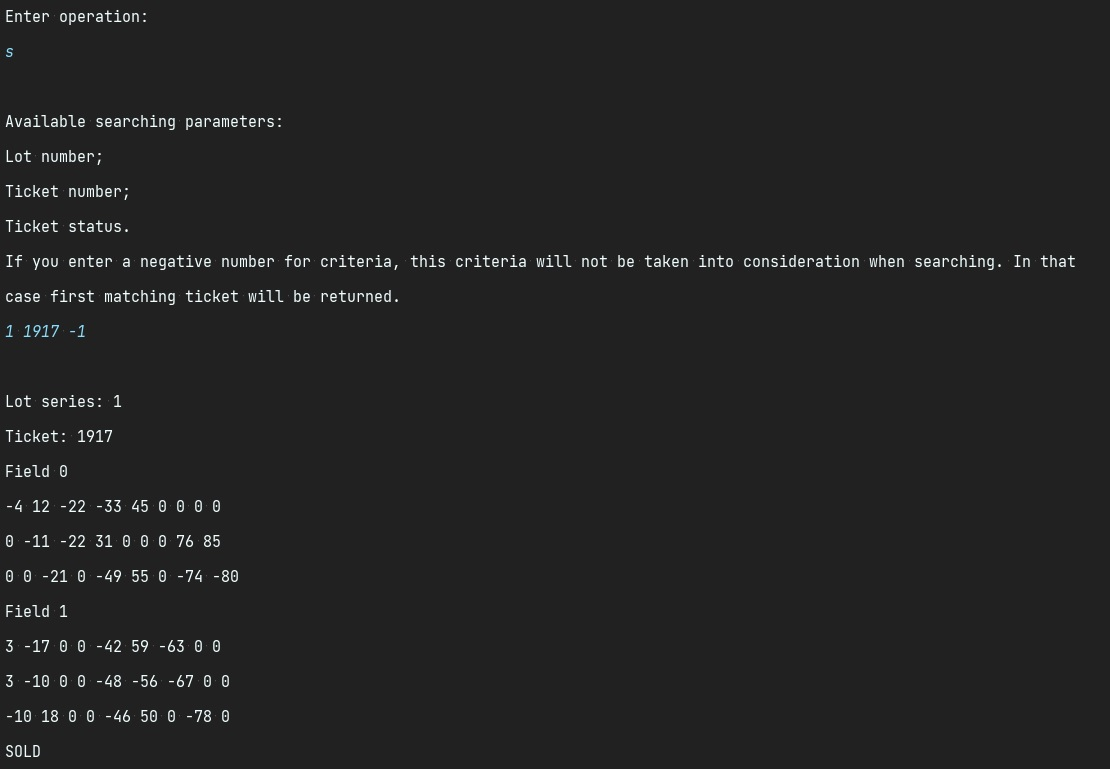
\includegraphics[width=\linewidth]{pictures/10}
  \caption{Пользователь вводит операцию поиска билета и программа находит билет согласно введенным параметрам.}
\end{figure}
\begin{figure}
  \centering
  \captionsetup{justification=centering,margin=1cm}
  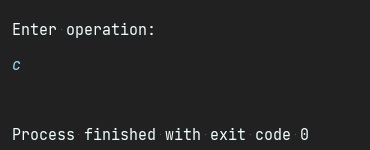
\includegraphics[width=\linewidth]{pictures/7}
  \caption{Пользователь звершает свою работу с программой, которая отработала без ошибок.}
\end{figure}
\begin{figure}[H]
  \centering
  \captionsetup{justification=centering,margin=1cm}
  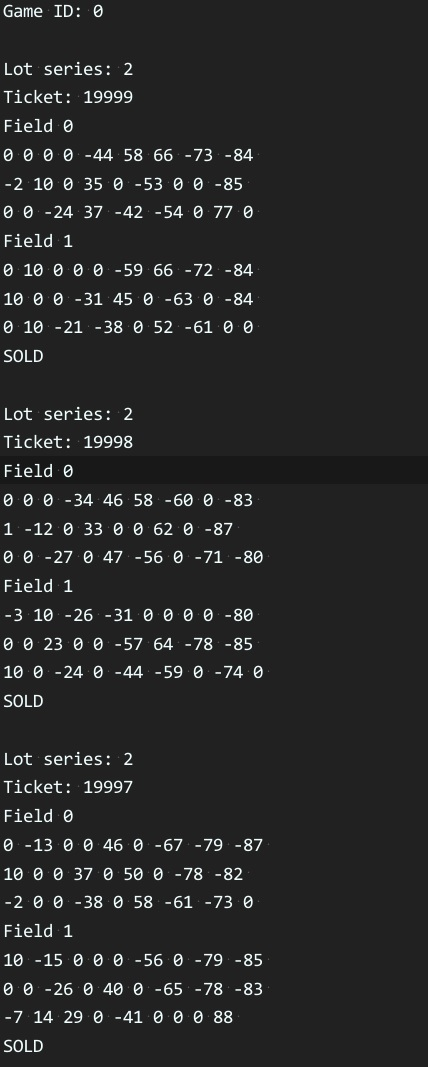
\includegraphics{pictures/8}
  \caption{Часть содержания файла output\_file.txt}
\end{figure}
\begin{figure}[H]
  \centering
  \captionsetup{justification=centering,margin=1cm}
  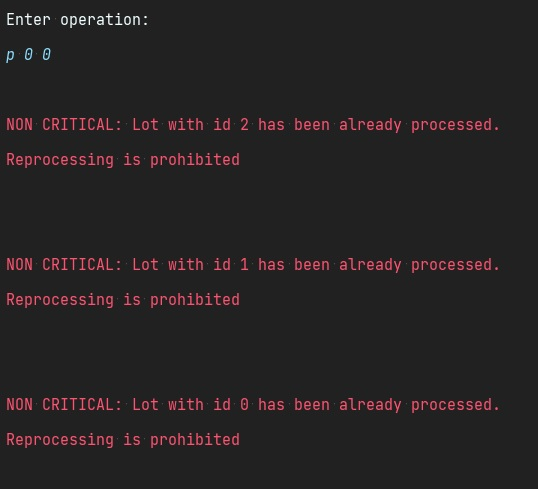
\includegraphics{pictures/11}
  \caption{Пример появления ошибок в процессе выполнения программы.}
\end{figure}
\clearpage

\section{Вывод}
Было разработано приложение для проведения лотереи и обработки соответствующих данных с использованием паттерна проектирования "Фабричный метод". Также в этом приложении был реализован интерфейс для односвязныйх списков forward_list и List с использованием паттерна "Декоратор" и продемонстрирована работа спроектированного приложения, симуляция проведения лотереи.
Коллекции forward_list и List были протестированы на достаточно больших количествах хранящихся в них объектов (>20 000 000 штук). В ходе тестов не было обнаружено какой-либо временной и сложностной разницы между реализациями односвязного списка. Сложность реализации вставки и удаления у обоих реализаций имеет линеюную сложность O(n). Поиск элемента в коллекции односвязного списка также имеет линейную сложность.
\newpage

\section{Литература}

\printbibliography

\clearpage

\section{Приложение}
\subsubsection{main.cpp}
\begin{minted}{C++}
#include <iostream>
#include <fstream>
#include <ctime>
#include "client_code.h"

using namespace std;

int main()
{
    ofstream ofp("output_file.txt");
    if(!ofp.is_open())
    {
        err_code=1;
        errCheck_Main();
    }

    srand(static_cast <unsigned>(time(nullptr)));

    if(clientCode(ofp))
        err_code=2;
    ofp.close();

    errCheck_Main();
}

\end{minted}
\subsubsection{client\_code.h}
\begin{minted}{C++}
int clientCode(ofstream &fp)
{
    SuperGenerator<FieldRusLot, LIST_IMPLEMENTATION> *super_gen = new SuperGeneratorRusLot<LIST_IMPLEMENTATION>();
    Game<FieldRusLot, LIST_IMPLEMENTATION> *game=super_gen->gen_game->getGame(*super_gen->gen_lot, *super_gen->gen_tic);   // Пример ввода: 0, 2, 2000000, 0.8

    cout << "Tickets were successfully generated.\n\n"
            "Available operations:\n"
            "'p' - enter process mode and id of lot to process. In zero mode id is useless;\n"
            "'o' - print winners;\n"
            "'f' - write processed data to output_file;\n"
            "'s' - search specific tickets in output_file;\n"
            "'c' - finish work and exit program.";
    char operation;
    int process_mode, number;
    bool proceed=true, p_not_blocked=true, s_not_blocked=false, o_f_not_blocked=false;
    while(proceed)
    {
        cout << "\n\nEnter operation:\n";                               // Пример ввода: p 0 0
        cin >> operation;
        switch(operation)
        {
            case 'p':
                if(p_not_blocked)
                {
                    cin >> process_mode >> number;
                    while((err_code = game->processGame(process_mode, number)) == -1)
                        cin >> process_mode;
                    if(err_code)
                    {
                        err_code=1;
                        p_not_blocked=false;
                        break;
                    }
                    o_f_not_blocked=true;
                }
                else
                    cout << BAD_ACCESS"Last calculation ended with errors.\n";
                break;

            case 'o':
                if(o_f_not_blocked)
                    game->printAllWinners();
                else
                    cout << BAD_ACCESS"Game has not been processed or processing has ended with errors.\n";
                break;

            case 'f':
                if(o_f_not_blocked)
                {
                    fp << *game;
                    s_not_blocked=true;
                    cout << "Processed data has been written to file.";
                }
                else
                    cout << BAD_ACCESS"Game has not been processed or processing has ended with errors.\n";
                break;

            case 's':
                if(s_not_blocked)
                {
                    if(!searchTickets(*game, super_gen->gen_tic->getTicket(0, 0, -1)))       // Пример ввода: 0 432 -1
                        err_code=1;
                }
                else
                    cout << BAD_ACCESS"Processed data has not been written to file.\n";
                break;

            case 'c':
                proceed=false;
                break;

            default:
                cout << "No such operation, try again.\n";
        }
    }
    delete super_gen; delete game;

    return errCheck_ClientCode();
}
\end{minted}
\subsubsection{functions.h}
\begin{minted}{C++}
int floatChanceToInt(float chance)
{
    chance*=100;
    if(chance>100)
        chance=rand() %100 +1;
    return (int)chance;
}

int foundDuplicate(int8_t *arr, int i, int number)
{
    i++;
    for(int j=0; j<i; j++)
        if(number==arr[j])
            return 1;
    arr[i-1]=number;
    return 0;
}

void getValues(int8_t arr[2][5])
{
    int i, min;
    for(i=0; i<5; i++)
        while(foundDuplicate(arr[0], i, rand() % 9)) {}
    for(i=0; i<5; i++)
    {
        if((min=(arr[0][i]+1)*10-10)==0)
            min=1;
        while(foundDuplicate(arr[1], i, rand() % 10+min)) {}
    }
}

\end{minted}
\subsubsection{components.h}
\begin{minted}{C++}
#include <algorithm>
#include <vector>
#include <cstdint>
#include <random>
#include <chrono>
#include "list_decorator.h"
#include "functions.h"

#define NUMBER_OF_KEGS 90

using namespace std;

template<class T>
class GeneratorTicket;
template <class T, template<class> class L>
class GeneratorLot;

class KegBag
{
private:
    vector<unsigned int> bag;
public:
    KegBag(unsigned &seed)
    {
        seed+=rand();                           // rand() прибавлен из-за того, что seed практически не меняется за время, достаточное для генерации нескольких билетов.
        for(int i=1; i<NUMBER_OF_KEGS; i++)
            bag.push_back(i);
        shuffle(bag.begin(), bag.end(), default_random_engine(seed));
    }
    void getKegs(vector<unsigned int> &vec, unsigned int amount)
    {
        vec.clear();
        for(int i=0; i<amount; i++)
        {
            vec.push_back(bag.back());
            bag.pop_back();
        }
    }

    friend const ostream& operator<<(ostream &out, const KegBag &keg_bag)
    {
        out << "Remaining kegs in bag:";
        for(auto it : keg_bag.bag)
            out << ' ' << it;
        return out;
    }
};

class Field
{
protected:
    unsigned long long row_count;
    unsigned long long col_count;
    int8_t **field;
public:
    Field(unsigned long long rows, unsigned long long cols) : row_count(rows), col_count(cols)
    {
        unsigned long long j;
        int8_t field_values_in_row[2][5];

        field=new int8_t *[row_count];
        for(unsigned long long i=0; i<row_count; i++)
        {
            field[i]=new int8_t[col_count];
            for(j=0; j<col_count; j++)
                field[i][j] = 0;

            getValues(field_values_in_row);
            for (j = 0; j < 5; j++)
                field[i][field_values_in_row[0][j]] = field_values_in_row[1][j];
        }
    }
    ~Field()
    {
        for(int i=0; i<row_count; i++)
            delete[]field[i];
        delete[]field;
    }
    friend const ostream& operator<< (ostream &out, const Field &fld);
    friend istream& operator>> (istream &in, Field &fld);
    template<class> friend class Ticket;
};

class FieldRusLot : public Field
{
public:
    FieldRusLot() : Field(3, 9) {}
};

const ostream& operator<< (ostream &out, const Field &fld)
{
    for(int i=0; i<fld.row_count; i++)
    {
        for(int j=0; j<fld.col_count; j++)
            out << (int)fld.field[i][j] << ' ';
        out << '\n';
    }
    return out;
}

istream& operator>> (istream &in, Field &fld)
{
    int tmp;
    for(int i=0; i<fld.row_count; i++)
    {
        for(int j=0; j<fld.col_count; j++)
        {
            in >> tmp;
            fld.field[i][j]=tmp;
        }
        in.get(); in.get();
    }
}

template <class T, template<class> class L> class Game;

template<class T>
class Ticket
{
protected:
    unsigned long long lot_number, ticket_number, status;
    vector<T> fields;
public:
    Ticket(unsigned long long lot_num, unsigned long long ticket_num, unsigned int field_count, unsigned int status) :
            lot_number(lot_num), ticket_number(ticket_num),
            fields(field_count), status(status) {}
    ~Ticket()
    {
        fields.clear();
    }
    int getStatus()
    {
        return status;
    }
    int processTicket(vector<unsigned int> &numbers, int vic_type)
    {
        int i, j;
        int counters[3] = {0};                                            // Проверяют строку, поле и билет на зачеркивание всех чисел в строке/поле/всех полях.
        for(auto &fld : fields)
        {
            counters[1]=0;
            for(i=0; i<fld.row_count; i++)
            {
                counters[2]=0;
                for(j=0; j<fld.col_count; j++)
                {
                    for(auto &num : numbers)
                    {
                        if(fld.field[i][j] < 0)
                            counters[2]++;
                        else if (num == fld.field[i][j])
                        {
                            fld.field[i][j]*=-1;
                            counters[2]++;
                            break;
                        }
                    }
                }
                if(counters[2]==5)
                {
                    if(vic_type==1)
                    {
                        status = 2;
                        return 1;
                    }
                    counters[1]++;
                }
            }
            if(counters[1]==3)
            {
                counters[0]++;
                if(vic_type==2)
                {
                    status = 3;
                    return 1;
                }
            }
        }
        if(counters[0]==2 && vic_type==3)
        {
            status = 4;
            return 1;
        }
        return 0;
    }
    friend ostream& operator<< (ostream &out, const Ticket<T> &tic)
    {
        out << "Lot series: " << tic.lot_number << '\n';
        out << "Ticket: " << tic.ticket_number << "\n";

        unsigned int field_count=tic.fields.size();
        for(int i=0; i<field_count; i++)
            out << "Field " << i << '\n' << tic.fields[i];

        switch(tic.status)
        {
            case 0:
                out << "UNSOLD";
                break;
            case 1:
                out << "SOLD";
                break;
            case 2:
                out << "1-st TOUR WINNER, SOLD";
                break;
            case 3:
                out << "2-nd TOUR WINNER, SOLD";
                break;
            case 4:
                out << "3-rd TOUR WINNER, SOLD";
                break;
        }
        out << '\n';
        return out;
    }
    friend istream& operator>> (istream &in, Ticket<T> &tic)
    {
        unsigned int size=tic.fields.size();
        char c;

        in.ignore(12);
        in >> tic.lot_number;
        in.ignore(8,' ');
        in >> tic.ticket_number;
        in.get(c);
        for(int i=0; i<size; i++)
        {
            in.ignore(20, '\n');                                          // Пропуск Field.
            in>>tic.fields[i];
        }
        in.get(c);
        switch(c)
        {
            case 'U':
                tic.status = 0;
                break;
            case 'S':
                tic.status = 1;
                break;
            case '1':
                tic.status = 2;
                break;
            case '2':
                tic.status = 3;
                break;
            case '3':
                tic.status = 4;
                break;
        }
        in.ignore(30, '\n');
    }
    template <class C, template<class> class L> friend Ticket<C> *searchTickets(Game<C, L> &game, Ticket<C> *tic);
    template <class, template<class> class> friend class Lot;
};

class TicketRusLot : public Ticket<FieldRusLot>
{
public:
    TicketRusLot(unsigned long long lot_num, unsigned long long ticket_num, unsigned int status) : Ticket(lot_num, ticket_num, 2, status) {}
};

template <class T, template<class> class L>
class Lot
{
private:
    bool was_processed;
    unsigned long long lot_number;
    KegBag keg_bag;
    ListBasicInterface<L, Ticket<T>*> lot_tickets;
public:
    Lot(unsigned long long num, unsigned long long num_of_tickets, unsigned int sale_chance, unsigned &seed, GeneratorTicket<T> &gen) : was_processed(false), lot_number(num),
                                                                                                                            keg_bag(seed)
    {
        for(unsigned long long i=0; i<num_of_tickets; i++)
            lot_tickets.push_front(gen.getTicket(lot_number, i,(rand()%100)<sale_chance));
    }
    ~Lot()
    {
        lot_tickets.clear();
    }
    template <class, template<class> class> friend class Game;
    friend const ostream& operator<< (ostream &out, Lot<T, L> &lot)
    {
        for(auto it = lot.lot_tickets.begin(); it!=lot.lot_tickets.end(); it++)
            out << **it << '\n';
        return out;
    }
};


template <class T, template<class> class L>
class Game
{
private:
    unsigned seed;
    unsigned long long id;
    unsigned long long count_of_lots;
    unsigned long long count_of_tickets;
    ListBasicInterface<L, Lot<T, L>*> lot_tickets;
    ListBasicInterface<L, Ticket<T>*> first_tour_winner_tickets;
    ListBasicInterface<L, Ticket<T>*> second_tour_winner_tickets;
    ListBasicInterface<L, Ticket<T>*> third_tour_winner_tickets;

    Game(GeneratorLot<T, L> &gen_lot, GeneratorTicket<T> &gen_tic) : seed(chrono::system_clock::now().time_since_epoch().count())
    {
        generationProceed(generationMenu(), gen_lot, gen_tic);      // Вызов меню для задания параметров генерации в качестве параметра для основной функции генерации
    }

    float generationMenu()
    {
        float sale_chance;
        cout << "Available generation parameters:\n"
                "Game id;\n"
                "Number of lots;\n"
                "Number of tickets in lot. Set this parameter to 0 if number of tickets in each lot should vary;\n"
                "Ticket sale chance (float). Set this parameter to number less than 0 if sale chance for tickets in each lot should vary.\t\t   "
                                            "Set this parameter to number greater than 1 to get random chance of sale for tickets in each lot.\n\n"
                "Enter parameters:\n";
        cin >> id >> count_of_lots >> count_of_tickets >> sale_chance;
        return sale_chance;
    }
    void generationProceed(float sale_chance, GeneratorLot<T, L> &gen_lot, GeneratorTicket<T> &gen_tic)
    {
        if(!count_of_tickets && (sale_chance<0))                                // Не хочется еще больше плодить сущностей и делать отдельную функцию.
        {
            unsigned long long num;
            for(int i=0; i<count_of_lots; i++)
            {
                cout << "Enter number of tickets and/or sale chance:\n";
                cin >> num >> sale_chance;
                lot_tickets.push_front(gen_lot.getLot(i, num, floatChanceToInt(sale_chance), seed, gen_tic));
            }
        }
        else if(!count_of_tickets)
        {
            unsigned long long num;
            for(int i=0; i<count_of_lots; i++)
            {
                cout << "Enter number of tickets and/or sale chance:\n";
                cin >> num;
                lot_tickets.push_front(gen_lot.getLot(i, count_of_tickets, sale_chance, seed, gen_tic));
            }
        }
        else if(sale_chance<0)
        {
            for(int i=0; i<count_of_lots; i++)
            {
                cout << "Enter number of tickets and/or sale chance:\n";
                cin >> sale_chance;
                lot_tickets.push_front(gen_lot.getLot(i, count_of_tickets, floatChanceToInt(sale_chance), seed, gen_tic));
            }
        }
        else
        {
            sale_chance = floatChanceToInt(sale_chance);
            for (int i = 0; i < count_of_lots; i++)
                lot_tickets.push_front(gen_lot.getLot(i, count_of_tickets, sale_chance, seed, gen_tic));
        }
    }
    void printWinners(ListBasicInterface<L, Ticket<T>*> &winner_tickets) const
    {
        if(winner_tickets.empty())
        {
            cout << "No winners!";
            return;
        }
        for(auto it=winner_tickets.begin(); it!=winner_tickets.end(); it++)
            cout << **it <<'\n';
    }
    int processTour(unsigned int n, auto &lot, ListBasicInterface<L, Ticket<T>*> &tour_winner_tickets, int victory_type, vector<unsigned int> &kegs)
    {
        for(int i=0; i<n; i++)                                       // Определение победителей происходит как по условию - после каждого хода.
        {
            (*lot)->keg_bag.getKegs(kegs, 1);
            for(auto tic : (*lot)->lot_tickets)
                if(tic->getStatus() == 1)
                    if(tic->processTicket(kegs, victory_type))
                        tour_winner_tickets.push_front(tic);
        }
    }
public:
    ~Game()
    {
        lot_tickets.clear();
        first_tour_winner_tickets.clear();
        second_tour_winner_tickets.clear();
        third_tour_winner_tickets.clear();
    };
    int processLot(long int lot_to_process, auto lot)
    {
        if(lot==lot_tickets.end())                                          // Проверка на нахождение номера тиража в списке тиражей.
        {
            auto lt=lot_tickets.begin();
            for (; lt!=lot_tickets.end(); lt++)
            {
                if (lot_to_process == (*lt)->lot_number)
                {
                    lot_to_process = -1;
                    break;
                }
            }
            if(lot_to_process != -1)
                return 1;
            lot=lt;
        }
        if((*lot)->was_processed)
            return 2;

        vector<unsigned int> kegs;
        (*lot)->keg_bag.getKegs(kegs, 5);
        cout << "\nProcessing lot with id " << (*lot)->lot_number << "\nProcessing first tour...\n";
        for(auto tic : (*lot)->lot_tickets)
            if(tic->getStatus()==1)
                tic->processTicket(kegs, 1);
        processTour(10, lot, first_tour_winner_tickets, 1, kegs);               // Первый параметр - количество вынимаемых бочонков в туре.
        cout << "Processing second tour...\n";
        processTour(30, lot, second_tour_winner_tickets, 2, kegs);
        cout << "Processing third tour...\n";
        processTour(15, lot, third_tour_winner_tickets, 3, kegs);

        (*lot)->was_processed=true;
        cout << (*lot)->keg_bag;

        return 0;
    }
    int processGame(int process_mode, unsigned long long number)
    {
        switch(process_mode)
        {
            case 0:
                for(auto lot=lot_tickets.begin(); lot!=lot_tickets.end(); lot++)
                    if((err_code=processLot((*lot)->lot_number, lot)))
                        errCheck_Components((*lot)->lot_number);
                break;
            case 1:
                if((err_code=processLot(number, lot_tickets.end())))
                    errCheck_Components(number);
                break;
            default:
                cout << "\nNo such mode, try again.";
                return -1;
        }
        return err_code;
    }
    void printAllWinners()
    {
        cout << "\n\nFirst tour winners:\n";
        printWinners(first_tour_winner_tickets);
        cout << "\nSecond tour winners:\n";
        printWinners(second_tour_winner_tickets);
        cout << "\nThird tour winners:\n";
        printWinners(third_tour_winner_tickets);
    }

    template <class, template<class> class> friend class GeneratorGameRusLot;
    friend const ostream& operator<< (ostream &out, Game<T, L> &game)
    {
        out << "Game ID: " << game.id << "\n\n";
        for(auto it=game.lot_tickets.begin(); it!=game.lot_tickets.end(); it++)
            out << **it;
        return out;
    }
};

template <class C, template<class> class L>
Ticket<C> *searchTickets(Game<C, L> &game, Ticket<C> *tic)           // Функция может быть также использована при работе с компонентами, так как возвращает указатель типа Ticket.
{
    ifstream fp("output_file.txt");
    if(!fp.is_open())
    {
        err_code=1;
        errCheck_Main();
    }
    fp.ignore(10,'\n');                                                    // Пропуск Game id.
    fp.get();

    long long criteria[3], initial_value=0, count_of_matching;
    cout << "\nAvailable searching parameters:\n"
            "Lot number;\n"
            "Ticket number;\n"
            "Ticket status.\n"
            "If you enter a negative number for criteria, this criteria will not be taken into consideration when searching. "
            "In that case first matching ticket will be returned.\n";
    cin >> criteria[0] >> criteria[1] >> criteria[2];
    for(long long i : criteria)
        if(i<0)
            initial_value++;
    do
    {
        count_of_matching=initial_value;
        fp >> *tic;
        if(tic->lot_number==criteria[0] && criteria[0]>-1)
            count_of_matching++;
        if(tic->ticket_number==criteria[1] && criteria[1]>-1)
            count_of_matching++;
        if(tic->status==criteria[2] && criteria[2]>-1)
            count_of_matching++;
        if(count_of_matching==3)
        {
            cout << '\n' << *tic;
            fp.close();
            return tic;
        }
    }
    while(fp.get()!=EOF);

    fp.close();
    cout << "Ticket not found.\n";
    return nullptr;
}
\end{minted}
\subsubsection{generators.h}
\begin{minted}{C++}
template<class T>
class GeneratorTicket
{
public:
    virtual Ticket<T> *getTicket(unsigned long long lot_num, unsigned long long ticket_num, unsigned int status) const = 0;
};

class GeneratorTicketRusLot : public GeneratorTicket<FieldRusLot>
{
public:
    Ticket<FieldRusLot> *getTicket(unsigned long long lot_num, unsigned long long ticket_num, unsigned int status) const override
    {
        return new TicketRusLot(lot_num, ticket_num, status);
    }
};

template <class T, template<class> class L>
class GeneratorLot
{
public:
    virtual Lot<T, L> *getLot(unsigned long long num, unsigned long long num_of_tickets, unsigned int sale_chance, unsigned &seed, GeneratorTicket<T> &gen) const = 0;
};

template <class T, template<class> class L>
class GeneratorLotRusLot : public GeneratorLot<FieldRusLot, L>
{
public:
    Lot<FieldRusLot, L> *getLot(unsigned long long num, unsigned long long num_of_tickets, unsigned int sale_chance, unsigned &seed, GeneratorTicket<T> &gen) const override
    {
        return new Lot<FieldRusLot, L>(num, num_of_tickets, sale_chance, seed, gen);
    }
};

template <class T, template<class> class L>
class GeneratorGame
{
public:
    virtual Game<T, L> *getGame(GeneratorLot<T, L> &gen_lot, GeneratorTicket<T> &gen_tic) const = 0;
};

template <class T, template<class> class L>
class GeneratorGameRusLot : public GeneratorGame<FieldRusLot, L>
{
public:
    Game<FieldRusLot, L> *getGame(GeneratorLot<T, L> &gen_lot, GeneratorTicket<T> &gen_tic) const override
    {
        return new Game<FieldRusLot, L>(gen_lot, gen_tic);
    };
};

template <class T, template<class> class L>
class SuperGenerator
{
public:
    GeneratorGame<T, L> *gen_game;
    GeneratorLot<T, L> *gen_lot;
    GeneratorTicket<T> *gen_tic;
    SuperGenerator(GeneratorGame<T, L> *gen_one, GeneratorLot<T, L> *gen_two, GeneratorTicket<T> *gen_three) : gen_game(gen_one), gen_lot(gen_two),
                                                                                                               gen_tic(gen_three){}
    ~SuperGenerator()
    {
        delete gen_game;
        delete gen_lot;
        delete gen_tic;
    }
};

template <template<class> class L>
class SuperGeneratorRusLot : public SuperGenerator<FieldRusLot, L>
{
public:
    SuperGeneratorRusLot() : SuperGenerator<FieldRusLot, L>::SuperGenerator(new GeneratorGameRusLot<FieldRusLot, L>(), new GeneratorLotRusLot<FieldRusLot, L>(),
                                                                            new GeneratorTicketRusLot()) {}
};
\end{minted}
\subsubsection{error\_check.h}
\begin{minted}{C++}
#define NON_CRITICAL "\nNON CRITICAL: "
#define CRITICAL     "\nCRITICAL: "

using namespace std;

static int err_code;            // Замена errno.

int errCheck_Components(unsigned int additional_information)          // Можно было упаковать в классы, но, по-моему, лучше так.
{
    switch(err_code)
    {
        case 1:
            cerr << NON_CRITICAL"Unable to find Lot with id " << additional_information << " in Game!\nProcessing of this lot will not begin.\n\n";
            break;
        case 2:
            cerr << NON_CRITICAL"Lot with id " << additional_information << " has been already processed.\nReprocessing is prohibited\n\n";
            break;
    }
}

int errCheck_ClientCode()
{
    switch(err_code)
    {
        case 1:
            cerr << NON_CRITICAL"Game processing operation ended with errors.\n\n";
            break;
        case 2:
            cerr << NON_CRITICAL"Search operation has returned nullptr.\n\n";
            break;
    }
    if(err_code)
        return 2;
    return 0;
}

void errCheck_Main()
{
    switch(err_code)
    {
        case 0:
            exit(0);
        case 1:
            cerr << CRITICAL"Failed to open output file.";          // Обьекты, наследуемые от класса исключений, при критических ошибках не используются.
            exit(1);
        case 2:
            cerr << NON_CRITICAL"Program has ended with some errors.";
            exit(2);
    }
}
\end{minted}
\subsubsection{list\_decorator.h}
\begin{minted}{C++}
template <class T>
struct Node
{
    T data;
    Node *next;
};

template <class T>
class List
{
private:
    Node<T> *head;
    Node<T> *temp;
public:
    List()
    {
        head=nullptr;
    }

    bool empty() const
    {
        return (head==nullptr);
    }
    void push_front(const T &data)
    {
        temp = new Node<T>;
        temp->data = data;
        if(empty())
            temp->next = nullptr;
        else
            temp->next = head;
        head = temp;
    }
    void pop_front()
    {
        if(!empty())
        {
            Node<T> *tmp=head;
            head=head->next;
            delete tmp;
        }
    }
    void clear()
    {
        if(empty())
            return;
        for(typename List<T>::iterator it=begin(); it!=end(); it++)
            delete *it;
    }

    class iterator
    {
    friend class List;
    private:
        const Node<T>* current;
    public:
        iterator() : current(nullptr) {}
        iterator(const Node<T>* p_node) : current(p_node) {}

        iterator& operator=(Node<T>* node)
        {
            this->current = node;
            return *this;
        }
        iterator& operator++()
        {
            if(current)
                current = current->next;
            return *this;
        }
        iterator operator++(int)
        {
            iterator iterator=*this;
            ++*this;
            return iterator;
        }
        bool operator==(const iterator& it) const
        {
            return current == it.current;
        }
        bool operator!=(const iterator& it) const
        {
            return current != it.current;
        }
        T operator*() const
        {
            return current->data;
        }
    };
    iterator begin() const
    {
        return iterator(head);
    }
    iterator end() const
    {
        return iterator(nullptr);
    }
};

template<template<typename> class Container, typename T>
class ListBasicInterface
{
private:
    Container<T> lst;
public:
    ListBasicInterface() = default;
    typename Container<T>::iterator begin()
    {
        return lst.begin();
    }
    typename Container<T>::iterator end()
    {
        return lst.end();
    }
    bool empty() const
    {
        return lst.empty();
    }
    void push_front(const T &data)
    {
        lst.push_front(data);
    }
    void pop_front()
    {
        lst.pop_front();
    }
    void clear()
    {
        lst.clear();
    }
};
\end{minted}
\cite{knuth-fa}
\cite{knuth-acp}
\cite{knuthwebsite}
\printglossaries

\clearpage

\end{document}